%!TEX root = ../prueba.tex

\section{Contexto}

En Zacatenco, como en la mayoría de zonas escolares en la Ciudad de México, existe una cantidad considerable de proveedores de servicios de alimentos y bebidas, los cuales a veces tienen un espacio dentro de las instalaciones de las escuelas y otras veces se ubican fuera de las mismas. Estos establecimientos se enfrentan día a día a grandes olas de clientes que los prefieren por sabor, ambiente o cercanía con el único fin de alimentarse durante su tiempo libre o tiempo de receso. Muchas veces, el personal de estos establecimientos no se da abasto en recursos y tiempo para atender a la mayoría de los clientes que los visitan.

\subsection{Identificación del Problema}

El problema que identificamos tras una lluvia de ideas fue el siguiente:\\

\begin{center}\textit{El tiempo que un cliente debe esperar para ser atendido y recibir su comida o botana en un servicio de cafetería sobrepasa su tiempo libre o de receso.}\end{center}

Encontramos las siguientes causas más comunes del problema que mencionamos anteriormente son las siguientes:
	\begin{itemize}
		\item Pocas personas atendiendo la caja o preparando la comida.
		\item Un control de recursos(alimentos) que no responde a la demanda a tiempo.
	\end{itemize}

Tras una breve encuesta a la comunidad de la Escuela Superior de Cómputo, encontramos las siguientes consecuencias del problema que mencionamos anteriormente:
	\begin{itemize}
		\item Un cliente siente enojo cuando no obtiene el producto que deseaba o quería en el momento en el que se formó.
		\item Un cliente se siente estresado al esperar en una fila muy larga.
		\item Un cliente le da preferencia a la competencia al tener menos personas esperando por sus pedidos.
	\end{itemize}
	
	
\subsection{Identificación de Stakeholders/Actores del Sistema}

Los stakeholders son aquellas personas que se verán afectadas de forma directa o indirecta por la realización y conclusión del proyecto. A lo largo de está sección se presentan a los roles que se han identificado y que van a interactuar de forma directa con el sistema utilizando la aplicación móvil o la aplicación web. Para representar a los stakeholders, se utiliza la especificación \textit{UML} para actores.\\

En la figura \ref{fig:organigrama} se muestra la estructura jerárquica y generalizada de una cafetería, esto con el fin de identificar, separar y priorizar los requerimientos de los actores del sistema y hacer la estimación correspondiente de tiempo y costos. El organigrama también nos permite definir parte del diagrama de actores del sistema bajo el cual se harán las relaciones correspondientes con las user stories que se pueden observar al finalizar el siguiente capítulo.

\begin{figure}[hbtp!]
	\begin{center}
		\fbox{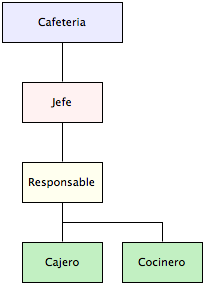
\includegraphics[width=0.3\textwidth]{img/organigrama}}
		\caption{Organigrama de una Cafetería}
		\label{fig:organigrama}
	\end{center}
\end{figure}


En la figura \ref{fig:actores} se muestra un diagrama en \textit{UML} que tiene como propósito representar cómo está dividido el sistema en función de los stakeholders identificados. A continuación se enlistan las observaciones más relevantes de este diagrama.
\begin{Citemize}
	\item La \getElementById[Stakeholder]{Persona} es un actor abstracto el cual tiene como principal objeto generalizar las funcionalidades a las que todos los actores del sistema tendrán acceso independientemente de su rol como por ejemplo iniciar sesión o recuperar su cuenta.
\end{Citemize}

\begin{figure}[hbtp!]
	\begin{center}
		\fbox{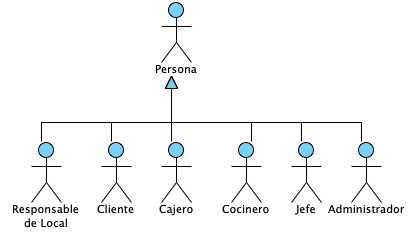
\includegraphics[width=0.5\textwidth]{img/actores}}
		\caption{Actores del Sistema}
		\label{fig:actores}
	\end{center}
\end{figure}

A continuación se hará la descripción formal de cada uno de los actores(ó stakeholders) del sistema. Esta descripción incluye un breve resumen del actor, sus responsabilidades en el sistema y el perfil que una persona debe cubrir para tener este rol.


\begin{Actor}{Persona}{Persona}{Un usuario es toda persona que va a interactuar con el sistema mediante la aplicación móvil o la aplicación web.}
	\item[Responsabilidades:] No aplica.
	\item[Perfil]:\hspace{1pt}
		\begin{itemize}
			\item Alumno de nivel medio superior, superior o posgrado del I.P.N. o de U.N.A.M.
			\item Docente de nivel medio superior, superior o posgrado del I.P.N. o de U.N.A.M.
			\item Personal externo en una unidad académica del I.P.N. o escuela de la U.N.A.M.
			\item Personal de una cafetería.
		\end{itemize}
\end{Actor}

\begin{Actor}{Jefe}{Jefe}{También conocido como \textbf{Dueño} es la persona que legalmente tiene derecho a utilizar el nombre de una franquicia para abrir uno o más locales en determinados espacios, dentro o fuera de una unidad académica del I.P.N. así como una escuela de otra Institución Educativa.}
	\item[Responsabilidades:] \hspace{1pt}
		\begin{itemize}
			\item Agregar al sistema a los empleados.
			\item Designar un responsable del local.
			\item Tomar desiciones ejecutivas que respondan a las demandas de su establecimiento con base en 			gráficas o datos estadísticos.
			\item Definir las horas de operación de un local.
		\end{itemize}
	\item[Perfil]:\hspace{1pt}
		\begin{itemize}
			\item Licenciatura.
			\item Responsable.
			\item Líder.
		\end{itemize}
\end{Actor}


\begin{Actor}{Administrador}{Administrador}{Es la persona que se encargará de desbloquear cuentas de usuario en el sistema así como de vigilar y mejorar las respuestas del sistema una vez sea puesto en producción.}
	\item[Responsabilidades:]\hspace{1pt}
		\begin{itemize}
			\item Desbloquear cuentas de usuario que estén bloqueadas.
		\end{itemize}
	\item[Perfil:]\hspace{1pt}
		\begin{itemize}
			\item Licenciatura en Computación, Ingeniería en Sistemas Computacionales o a fin concluida.
			\item Conocimientos Avanzados en Tunning y Performance de bases de datos.
		\end{itemize}
\end{Actor}


\begin{Actor}{ResponsableDeLocal}{Responsable de Local}{Es la persona encargada de administrar la información de una cafetería como lo es el nombre de la cafetería, ubicación, escuelas a las que generalmente atiende y los productos en inventario.}
	
	\item[Responsabilidades:]\hspace{1pt}
		\begin{itemize}
			\item Vigilar que los reglamentos internos y de salubridad se cumplan y hacer cumplir las sanciones correspondientes.
			\item Administrar la información de los productos que se venden en su local.
			\item Vigilar que el proceso de surtido se lleve a cabo de forma correcta.
		\end{itemize}
	
	\item[Perfil:]\hspace{1pt}
		\begin{itemize}
			\item Experiencia en administración de empresas.
			\item Responsable.
			\item Honesto.
		\end{itemize}
	
\end{Actor}
		
\begin{Actor}{Cocinero}{Cocinero}{Es una persona que pertenece a una o más cafeterías y que tiene como principal responsabilidad atender pedidos y cocinarlos o delegarle esta responsabilidad a otro cocinero dentro de la misma cafetería.}
	
	\item[Responsabilidades:] \hspace{0.5cm}
		\begin{itemize}
			\item Monitoreo, control y conservación de los insumos de la cocina.
			
			\item Colaborar en la planificación de menús.
			
			\item Ayudar a administrar los costos e inventario.
			
			\item Dividir, conducir y organizar el trabajo con otros miembros del staff en la preparación de las ordenes.
			
			\item Iteractuar con el proveedor del servicio.
			
			\item Atender y preparar los pedidos solicitados por los clientes.
		\end{itemize}
	
	\item[Perfil:] \hspace{0.5cm}
		\begin{itemize}
			\item Excelentes habilidades de comunicación.
			
			\item Buenos estándares de higiene.
			
			\item Organizado y metódico.
			
			\item Experiencia en cáterin.
		\end{itemize}
	
	\end{Actor}
	
	
	\begin{Actor}{Cajero}{Cajero}{Es una persona que pertenece a una o más cafeterías y que tiene como propósito cobrar los pedidos de los clientes.}
	
	\item[Responsabilidades:] \hspace{0.5cm}
		\begin{itemize}
			\item Recibir dinero en efectivo, de requerirlo realiza arqueos de caja.
			
			\item Es el responsable directo de dinero en efectivo.
			
			\item Registrar operando una caja los movimientos de entrada y salida de dinero.
			
			\item Informar a su superior los movimientos diarios de la caja.
			
			\item Mantener en orden el equipo y sitio de trabajo, reportando cualquier anomalia.
			
			\item Manejar un grado de confidencialidad sobre las transacciones bajo.
		\end{itemize}
	
	\item[Perfil:] \hspace{0.5cm}
		\begin{itemize}
			\item Excelentes habilidades de comunicación , para atención al cliente.
			
			\item Habilidades numericas.
			
			\item Actitud de servicio.
			
			\item Proactivo.
			
			\item Responsable.
			
			\item Buena gestión de tiempo.
		\end{itemize}
	
	\end{Actor}

	\begin{Actor}{Cliente}{Cliente}{Es cualquier persona(alumno, profesor, personal externo) que consume o adquiere los productos de una cafetería para consumirlos.}
	
	\item[Responsabilidades:]\hspace{1pt}
		\begin{itemize}
		\item Confirmar los pedidos que se realicen en el sistema.
		\item Realizar el pago correspondiente por los productos solicitados y consumidos.
		\end{itemize}
	\item[Perfil:]\hspace{1pt}
		\begin{itemize}
			\item Alumno de nivel medio superior, superior o posgrado del I.P.N. o de U.N.A.M.
			\item Docente de nivel medio superior, superior o posgrado del I.P.N. o de U.N.A.M.
			\item Personal externo en una unidad académica del I.P.N. o escuela de la U.N.A.M.
		\end{itemize}
	\end{Actor}